\ylDisplay{Takisti} % Ülesande nimi
{Jonathan Kalmus} % Autor
{piirkonnavoor} % Voor
{2018} % Aasta
{P 6} % Ülesande nr.
{3} % Raskustase
{
% Teema: Elektriõpetus

\ifStatement
Juku tahab mõõta tundmatu takisti väärtust. Selleks ühendab ta takistiga rööbiti voltmeetri ning ampermeetri jadamisi nagu näidatud joonisel. Ampermeetri näit $I = 15$ $m_A$ ning voltmeetri näit $U = 5$  $V$. Voltmeetri takistus $R_V = 1000$ $\Omega$. Leidke tundmatu takisti väärtus.
\begin{center}
	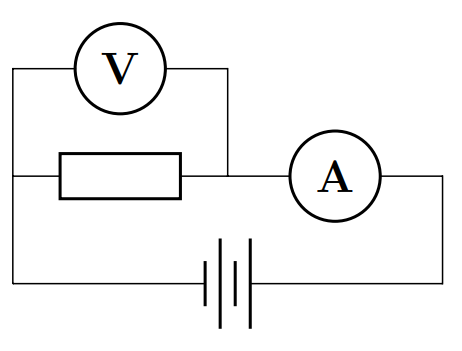
\includegraphics[width=0.5\linewidth]{2018-v2p-06-yl.png}
\end{center}
\fi

\ifHint
Takisti väärtus on voltmeetri sisetakistusega samas suurusjärgus ning seetõttu ei saa seda ignoreerida.
\fi


\ifSolution
Esimesel hinnagul $R \approx \frac{U}{I} \approx \frac{5}{0,015} \approx 333$ $\Omega$ on takisti väärtus voltmeetri sisetakistusega samas suurusjärgus ning seetõttu ei saa seda ignoreerida. Voltmeetri näit on täpne, sest on ühendatud takistiga otse rööbiti, kuid ampermeeter mõõdab summarset voolu, mis läheb läbi takisti ja voltmeetri. Läbi voltmeetri läheb $I_V = \frac{U}{R_V}$ , seega läbi takisti minev tegelik vool on $I_T = I - I_V$. Takisti tegelikuks väärtuseks saame
\begin{center}
$R_T = \frac{U}{I - I_V}$.
\end{center}
\begin{center}
$R_T = \frac{5}{0,015 - \cfrac{5}{1000}} = 500$ $\Omega$.
\end{center}
\fi
}